\chapter{SMS} %% change
\label{chapter_5} %% change
\graphicspath{ {./chapter-5/figures/} }  %% change
\captionsetup[figure]{labelfont=bf}
\captionsetup{margin=1.5em}
\captionsetup[table]{labelfont=bf}
%% The following annotation is customary for chapter which have already been
%% published as a paper.
\blfootnote{Parts of this chapter have been published in Optics Express \textbf{25}, 32474 (2018) \cite{HouSMS2018}.}

%% It is only necessary to list the authors if multiple people contributed
%% significantly to the chapter.
%\authors{Albert {\titleshape Einstein}}

%% The '0pt' option ensures that no extra vertical space follows this epigraph,
%% since there is another epigraph after it.
% \epigraph[0pt]{
%   A journey of a thousand miles begins with a single step
% }{Laozi}

% \epigraph{
%     Sample quotes
% }{author}

% \begin{abstract}
% Previous researches have shown that different solutions of the optical system can be found using saddle point based method for some simplified cases\cite{PascalTriplet2009}. It is important, however, to study whether the saddle point based method still perform well in practical lens design problems. To study this, we chose to start with a relative simple example.
% \end{abstract}

% %% Start the actual chapter on a new page.
% \newpage

\noindent 


%%%%%%%%%%%%%%%%%%%%%%%%%%%%%%%%%%%%%%%%%%% Section 1 %%%%%%%%%%%%%%%%%%%%%%%%%%%%%%%%%%%%%%%
\section{Introduction}
% repeat how the optical is done conventionally. Simple systems are determined by forward model analysis. The result from the simple model is then used as starting point for designing systems with more complexity.  
Choosing a sufficient good staring point is crucial to every kind of optical design. For a simple systems with a limited amount of optical elements, analytical method such as paraxial calculation or aberration analysis can be used to determine a starting point. Afterwards, the system is optimized with a design software in order to fulfill various constraints and performance requirements. These design solutions are documented either in lens design books \cite{book:Kingslake}\cite{book:SmithModernOpticalEngineering}\cite{book:FisherOpticalSysDesign} or in various patents. For system needs to meet demanding requirements where more design freedom is needed, the already documented design solutions form the selecting space for such starting point. 

There are various method to introducing design freedoms. In the context of designing rotational symmetric imaging systems, the typical ways are adding lens elements or using aspheric surfaces.  

%https://www.osapublishing.org/optica/fulltext.cfm?uri=optica-8-2-161&id=447006 freeform review

%% do I need this short para??
For systems mainly consist of spherical elements, we have shown in the previous chapters that the Saddle Point Construction method is helpful to systematically and rapidly scan through the complicated network of minima and saddle points. 

% Talking about the other aspect of the work 
Besides using additional lens elements, another aspect to increase the design parameter space is to introduce freedom in the existing lens surfaces. One way to realize it is by making the spherical surfaces into aspheric surfaces. They permit new dimensions in optical performance by eliminating aberrations without added weight and size, thus fulfilling the need for an ever-increasing performance balanced with an equal desirable goal of ever smaller and lighter optics. Experience shows that aspheric surface are often more challenging to manufacture and incorporate into design than the conventional spherical surfaces because of their complex geometric shape. Nonetheless, provided the added benefit, the development of precise manufacturing techniques makes aspheric surfaces no longer a luxury and therefore can be encountered quite often in modern designs. 
% continue to discuss the design with aspheric surfaces
For optical systems with few mild aspheric surfaces described by a small polynomial order, the traditional techniques may provide many useful solutions. However, when more complex systems with many aspheric surfaces with a large number of free parameters are considered, the optimization approach can easily get trapped in a poor local minimum (e.g., M2 in Figure \ref{fig: fig1_landscape}(a)) when the starting point (S2 in Figure \ref{fig: fig1_landscape}(a)) is far from the good local minimum of interest (M1 in Figure \ref{fig: fig1_landscape}(a)). In such cases, the designer´s experience is often a crucial factor when trying to get out of a poor minimum in search for a good solution. For instance, optimization is initially constrained to a lower dimension subspace, by optimizing only the low order coefficients. When a local minimum in the constrained subspace is reached (e.g., M in Figure \ref{fig: fig1_landscape}(b)), the subspace dimension is increased by unfreezing some higher-order coefficients. In the larger dimension subspace, that design is no longer a minimum and optimization can progress again, as illustrated in Figure \ref{fig: fig1_landscape}(b). When the number of variables is large, this change of the parameter subspace dimension can be done in various ways. Depending on the experience of the designer, which and how many variables are chosen in each step to optimize the system can be very different. 
%% describing the sequence of using variables affects the results since there is no control on the basin of attraction it stays. 
Different design strategies usually end up in different local minima. Several global optimization methods such as genetic algorithms \cite{Moore1999}, evolution strategies \cite{Nagar:18}, particle swarm \cite{MenkeParticleSwarm} and simulated annealing \cite{Forbes1991} have been adapted to different optical design problems to avoid getting trapped in a local minimum. However, these methods are based on generally applicable mathematical models, and designers understand little about the optical systems behind them. Another method known as saddle point construction (SPC) method uses a systematical approach to find solutions in the design landscape and helps to get out of bad local minima \cite{BociortSPCSexplained}\cite{HouSimple16}.
%% back in discussing these optimization method again
 
\begin{figure}[h!]
    \centering
    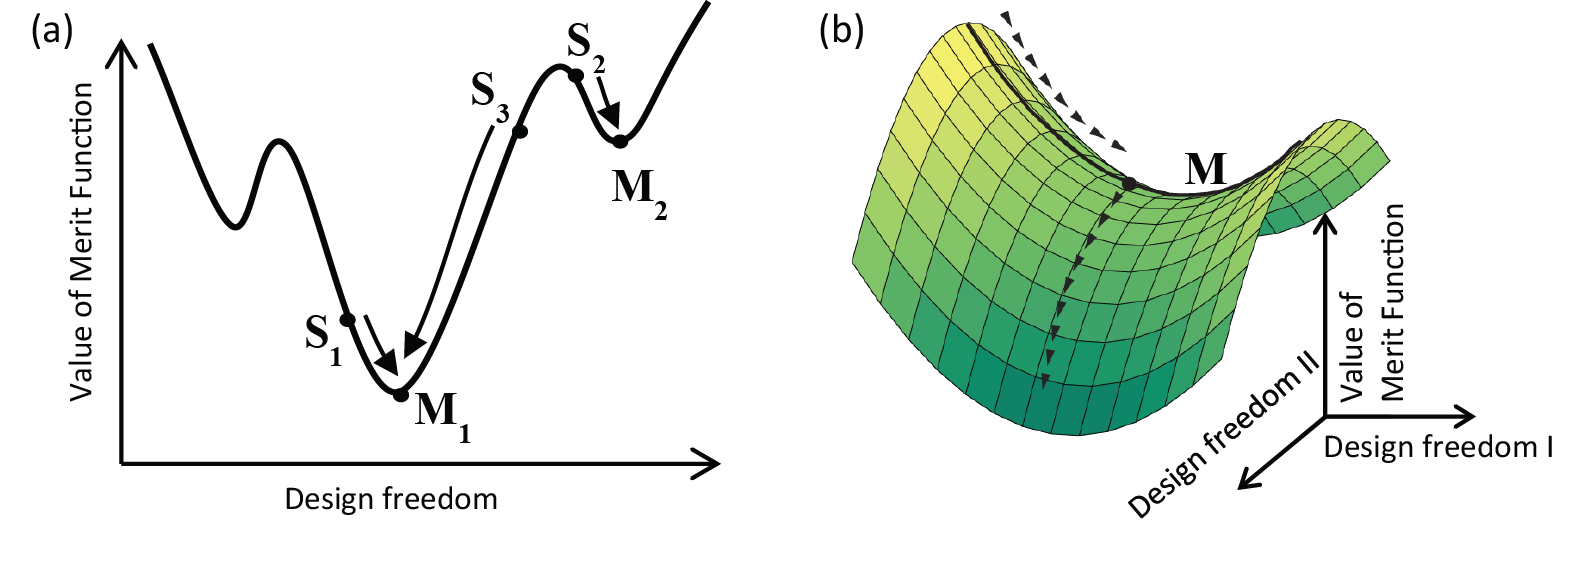
\includegraphics[width=0.8\textwidth]{chapter-5/figures/Figure1_landscape.png}
    \caption{An illustration of an optical design landscape in 2D (a) and 3D (b). }
    \label{fig: fig1_landscape}
\end{figure}
%% different than optimization method, SMS is a way to determine a starting point directly with aspheric surfaces. 
Alternatively, the Simultaneous Multiple Surfaces (SMS) method is a direct method that allows to find a better starting point (like S1 in Figure \ref{fig: fig1_landscape}(a)) \cite{WangThesis}\cite{LinWang12OE} and progress with it with a single step optimization (varying all parameters). Even though SMS is capable of designing good aspheric imaging systems, there is no study comparing it directly with other design strategies and describing the characteristics of different methods.

%Consider the context in this chapter. 
In this chapter, we consider rotationally symmetric designs, for which SMS 2D is used \cite{book:ChavesNonimagingOptics}. SMS 2D may utilize rays in the meridian plane or skew rays \cite{LinWang2011}, but in any case, obtaining a 2D profile of the surfaces. The method involves simultaneous calculation of N optical surfaces using N one-parameter bundles of rays for which specific conditions are imposed. The number of ray bundles can be greater than the number of surfaces to design when the footprints of the design bundles do not occupy the full SMS surfaces, as demonstrated in \cite{BenitezSPIE2014}\cite{FDuerrOE2013}\cite{FDuerrOE12}. SMS also has a freeform version called SMS 3D. However, these cases are not discussed in this paper. 
We start by briefly describing the SMS method applied in this paper. Then the design obtained with SMS is used as a starting point, followed by a single-step optimization of all parameters. The final design is compared with other designs obtained using spherical starting point and single-step, two-steps, stepwise and global optimizations. Two designs are considered, a simple one and a slightly more difficult one, with a larger aperture and wider field.
%%%% come back to check later 2021/03/02
\section{Starting point with the SMS method}
The standard SMS procedure for designing aspheric surfaces involves only meridian rays. It consists of two steps: selection of central segments of the surfaces and recursive generalized Cartesian oval calculation \cite{LinWang2011}\cite{MinanoOE09}. We will focus on SMS designs using only meridian rays. Skew rays are then controlled in a subsequent optimization. 

The illustration in Figure \ref{fig: sms_2d_explain} gives an example of how SMS works. The figure shows one of the approaches on how to design a two-surface aspheric imaging system. The following aspects need to be defined as the starting conditions: 1) Coordinates of the object points (\textbf{O1} and \textbf{O2}) and image points (\textbf{I2} and \textbf{I1}). The points in each pair are symmetric to each other with respect to the optical axis. 2) Vertex position (\textbf{P0}) of one of the surfaces and its normal (along the optical axis); thickness of the lens (it is approximated by the projection of \textbf{P0-P1} on the optical axis in Figure \ref{fig: sms_2d_explain}). 3) The refractive indices of the lens (\textit{n'} and the medium outside the lens \textif{n0}).

With all the above parameters defined, the SMS starts with tracing the ray from \textbf{O1} to \textbf{P0}. Then the ray is refracted to \textbf{P1}, then to \textbf{I1}(the normal at \textbf{P1} can now be calculated). Once the first complete ray is traced from \textbf{O1} to \textbf{I1}, the optical path distance (OPD) from \textbf{O1} to \textbf{I1} is known. Because of the symmetry, a perfect imaging system will produce the OPD from \textbf{O2} to \textbf{I2} identical to that from \textbf{O1} to \textbf{I1}. When tracing the ray from \textbf{I2} to \textbf{P1}, the refracted angle of the ray is known. Given the OPD and the end point as \textbf{O2}, the position of \textbf{P2} and the local normal can be calculated. 

Now, it is clear that the next step would be tracing the ray from \textbf{O1} to \textbf{P2}. The aforementioned steps can be iterated such that a chain of points is constructed. These points are positioned sparsely on the chain. To get dense sampled points, a curve can be interpolated with two neighboring points (e.g.  \textbf{P0} and \textbf{P2}) and their normals. A new point can be selected on this curve with its normal. Starting with the new point, we can perform the ray-tracing step again to create denser sampled points filling the gap between the original two points. The same procedure can be repeated with all the sparse points firstly created. After the dense sample points are available on both sides, surfaces can be created by fitting these points. 

This is only a brief explanation to show the concept of SMS. More details on different techniques for starting conditions, surface fitting and constructions are well explained in \cite{book:ChavesNonimagingOptics}.

\begin{figure}[h!]
    \centering
    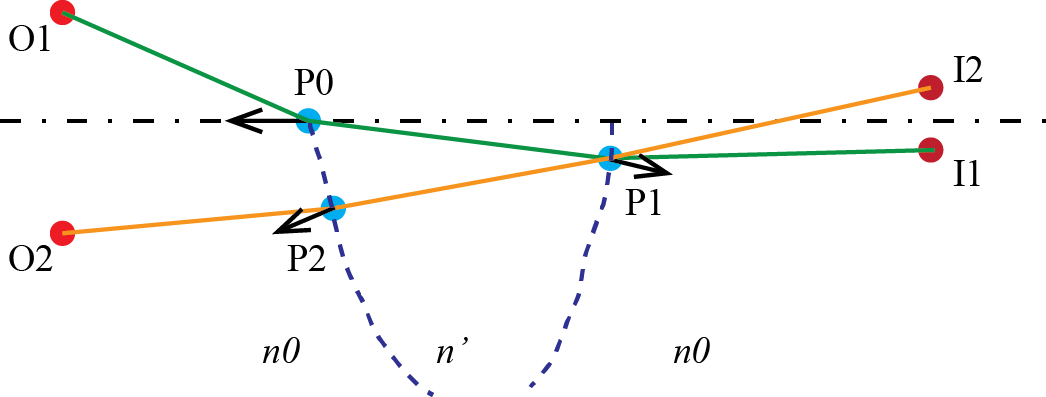
\includegraphics[width=0.85\textwidth]{chapter-5/figures/Figure_sms_explain_2D.png}
    \caption{Illustration of an SMS process to simultaneously construct two surfaces.}
    \label{fig: sms_2d_explain}
\end{figure}

In this chapter, two designs are studied. Both designs consist of four aspheric surfaces. The two designs are distinguished by the F/Number (aperture size) and the FOV where a smaller F/Number and larger FOV is considered as a more demanding design. With the SMS 2D approach, four meridian bundles were used. It is different from the two surfaces case in the way that the starting conditions include the parts of the surfaces near the axis, which are calcuated with paraxial optics \cite{MinanoOE09}. In this case, the four meridian ray bundles selected for the SMS design correspond to the rays emitted from four object points placed symmetrically about the optical axis at infinity. The image points are located in the same way at a finite distance to match the specified focal length. The field angles associated with the object points are selected so that their root mean square 2D (RMS2D) distribution curves (defined as the RMS spot diameter calculated using only meridian rays in the field) present a constant ripple over the field of view as shown in the right plot in Figure \ref{fig: fig2_SMSdesignedSys} and explained in detail in \cite{LinWang12OE}. 
Applying a standard SMS 2D procedure, for the design directions we simultaneously calculate the set of points and normals. SMS profiles are then fitted into a Forbes Qcon polynomial \cite{ForbesOE07}, which will be introduced into the CODE V software. This system is now ready to be optimized for the whole field of view, as in the example shown in Figure \ref{fig: fig2_SMSdesignedSys}. 

\begin{figure}[h!]
    \centering
    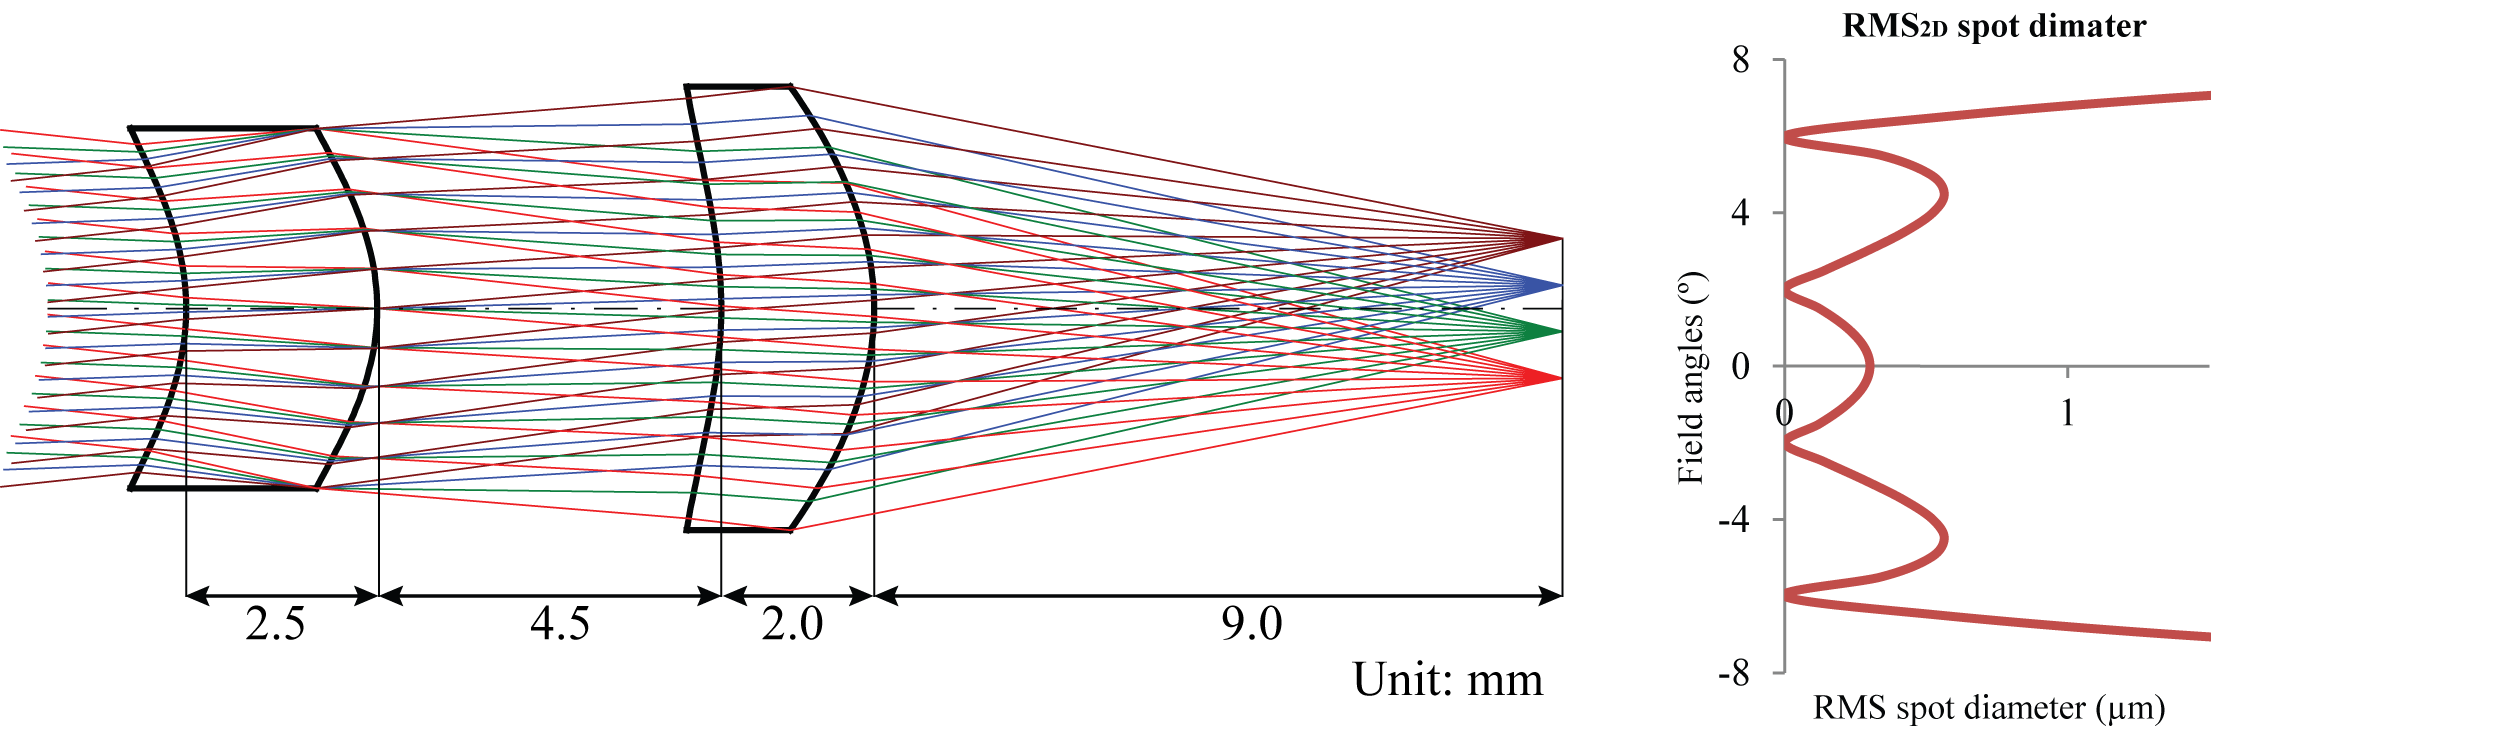
\includegraphics[width=1\textwidth]{chapter-5/figures/Fig2_SMSdesignedSystem.png}
    \caption{SMS 2D design introduced to CODE V after fitting the surfaces to Forbes Qcon polynomials. The change of the spot diameter through the fields is shown on the right side. 
An aperture stop is positioned at the right surface of the first lens element (when counting from left to right).  }
    \label{fig: fig2_SMSdesignedSys}).
\end{figure}

\section{Comparing the results of different design approaches}
Two lens systems were designed and optimized for monochromatic light ($\lambda$= 587.56 nm) using the SMS method and other approaches mentioned in the introduction. Both lenses are made of PMMA (n = 1.4918 at the used wavelength) and have four aspheric surfaces in total. The two systems are referred as system 1 and system 2 where their specifications are given in Table. \ref{table: SMS_SystemSpec}. The object is located at infinity. System 1 has both a smaller field of view (FOV) and aperture, and system 2 has both a larger FOV and aperture. 

\begin{table}[h!]
    \centering
    \captionsetup{justification=centering}
    \caption{System Specification}
    \label{table: SMS_SystemSpec}
    \vspace{-1em}
    \begin{adjustbox}{max width=\textwidth, center}
    \begin{tabular}{m{2cm} >{\centering\arraybackslash}m{3cm} >{\centering\arraybackslash}m{3cm} >{\centering\arraybackslash}m{3cm} >{\centering\arraybackslash}m{3cm}}
    \hline
     & \textbf{Image F/Number} & \textbf{Effective Focal Length (EFL)} & \textbf{Maximum Half Field of View (MHFOV)} & \textbf{Position of the Aperture Stop}\\
    \hline
    \textbf{System 1} & 2.24 & 8.60 mm & 7.50$^{\circ}$ & At surface 2 \\[1em]
    \textbf{System 2} & 1.77 & 10.60 mm & 11.50$^{\circ}$ & Air-space between the two lenses\\
    \hline
    \end{tabular}
    \end{adjustbox}
\end{table}

Three design approaches are used for the comparison: 1) SMS design with a subsequent one-step optimization; 2) optimization from a spherical system and adding aspheric coefficients, either with multiple coefficients in one-step, two-steps (each step with multiple coefficients) or one-by-one (stepwise, only one coefficient per step); 3) global optimization with Global Synthesis (GS) in CODE V. Since we do not intend to compare different global optimization algorithms in this paper, we choose for comparison with SMS only GS that is known to perform very well in comparison with other global optimization and search methods in lens design \cite{KuperGO1992}\cite{ShaferComPhy1994}. For comparison, the systems designed all use Qcon polynomials to represent the aspheric surfaces. The variables are the curvatures, conic constants and the coefficients of the Qcon polynomials. To better represent the surface constructed by the SMS method, we use up to the 12th order for system 1, and 16th order for system 2. The vertices are fixed in all cases. For non-GS optimization, we use the default CODE V transverse ray aberration merit function (MF). Two types of constraints are used. One is to constrain the effective focal length (EFL), and the other is to keep the normalization radii of the surfaces to a value exceeding the size of the surface aperture by $5\%$. The local optimization is done within CODE V based on a damped least square method. Vignetting was readjusted every 20 cycles, since the surface shape may vary significantly during the optimization process. Iterations are stopped when the MF value drops to less than $1^{-5} \mu m^2$ (convergence is then assumed). For GS optimization, the same MF and constraints are applied. However, vignetting can only be adjusted after the GS is finished. 

\begin{figure}[h!]
    \centering
    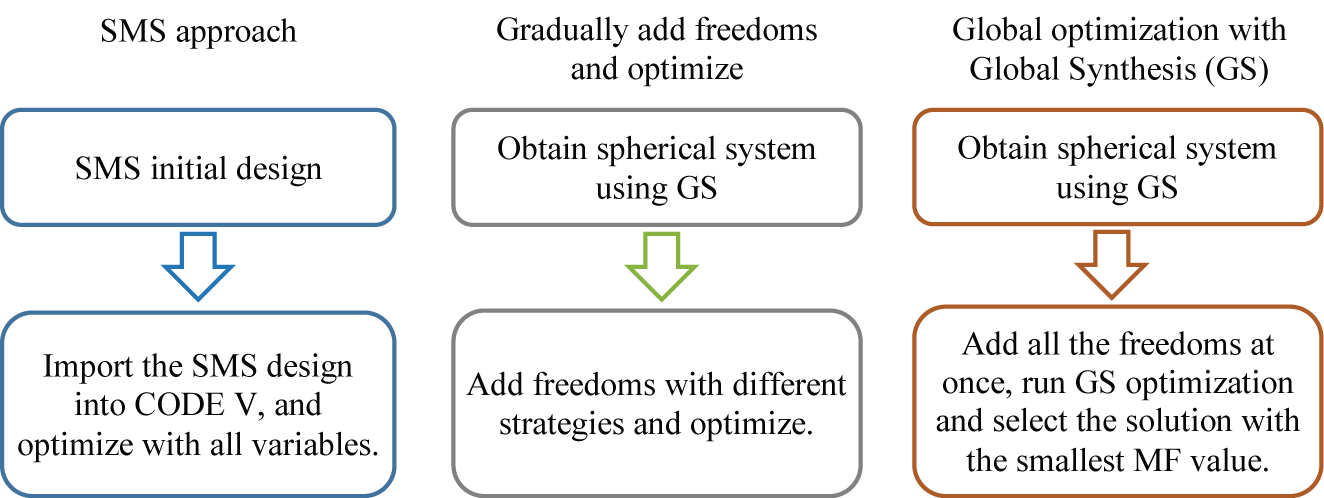
\includegraphics[width=0.8\textwidth]{chapter-5/figures/Fig3_flowchart.png}
    \caption{Flowchart for our different design approaches.}
    \label{fig: fig3_flowchart}
\end{figure}

The SMS 2D procedure enforces stigmatic imaging for meridian rays at a few discrete design fields. After the system is designed with SMS, it is imported into CODE V to be optimized for better performance throughout the whole field of view and the full pupil. The surface parameter of the two SMS constructed systems are given in Table \ref{table: chap5 - sys1 - SMS} and Table \ref{table: chap5 - sys2 - SMS} in the appendix. The left flowchart in Figure \ref{fig: fig3_flowchart} shows the design flow with SMS. 

\begin{figure}[h!]
    \centering
    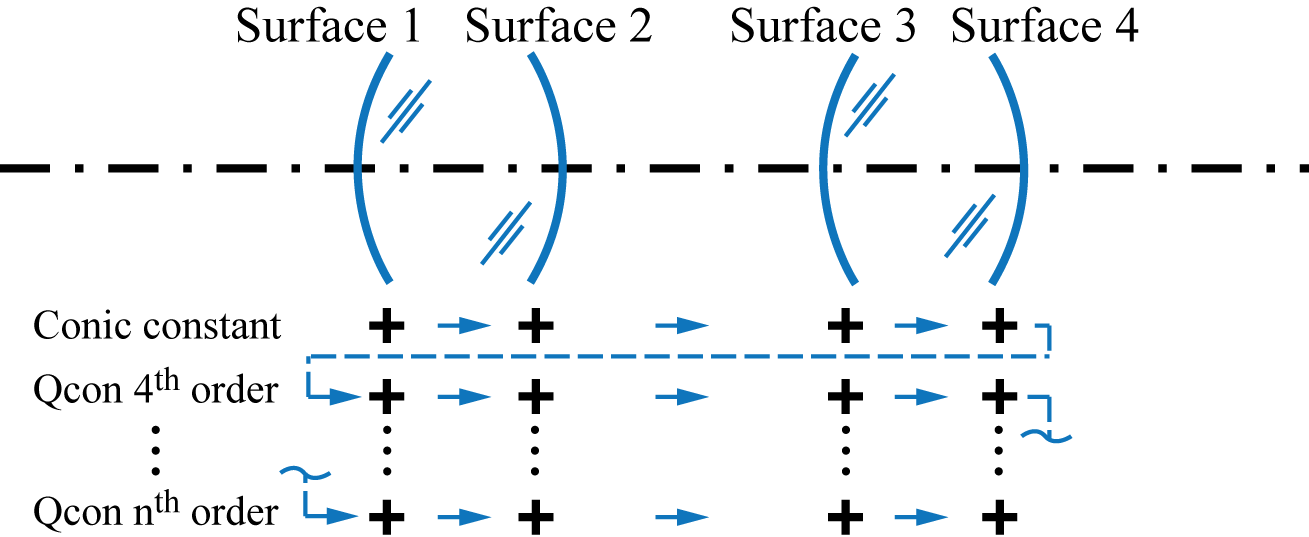
\includegraphics[width=0.8\textwidth]{chapter-5/figures/Figure4_stepwise.png}
    \caption{The strategy for stepwise optimization. The blue shapes represent the optical surfaces. Each cross represents a freedom on the surface described by the Qcon polynomial. The blue arrows indicate how the freedoms are added step by step up to the highest order coefficients used for Qcon polynomial. }
    \label{fig: fig4_stepwiseflow}
\end{figure}


The second approach is conventional and intuitive. We start with a good spherical system. This system is the only solution when spherical surfaces are used, and it is confirmed by GS of CODE V. Next, the aspheric coefficients are added as new variables. There are different strategies for adding variables to the system. The direct way is to free all the variables at once and optimize. For an optimization landscape with multiple minima, the optimized solutions will depend on the chosen starting point. Designers will not have control of the optimization route, and it is easy to get trapped in a poor local minimum. A common practice of experienced designers is adding variables step by step. In this paper, we apply three different strategies for adding new variables: a single-step optimization, a two-steps optimization, and an extensive stepwise approach. A two-steps approach is initiated by adding all the conic coefficients at once and then optimizing to a local minimum with conic surfaces. Subsequently, the higher-order coefficients of Qcon polynomial are added all together and optimized. The stepwise approach requires more steps by adding one freedom and then optimize each time: We start by freeing the conic constant on surface 1. After optimization, new freedom is added on the surface following the previous one, as shown in Figure \ref{fig: fig4_stepwiseflow}. Surface 1 with higher-order coefficient follows after surface 4 with lower-order coefficient. In practice, one can add the freedom to the system in several ways, keeping in mind that on each surface, the coefficients should be added from low order to high order. Since it is not known which stepwise strategy will lead to a better solution, in this paper, we choose an easy stepwise strategy for demonstration.  
In addition to the two approaches mentioned above, a global optimization method based on CODE V’s GS is used for comparison as well. The proprietary algorithm of GS can help the designer to automatically explore the solution space and synthesize new configuration from (nearly) arbitrary starting point \cite{codevmanual}. To apply GS, we use the spherical system mentioned above as a starting point. All the freedoms are added at once to the system. GS is executed with constraints on EFL and normalization radii. A time limit of two hours is set for the GS (i. e. GS stops after two hours if it is not finished). The resulting system with a reasonable system shape and the smallest MF value is chosen for the comparison. 

\begin{figure}[h!]
    \centering
    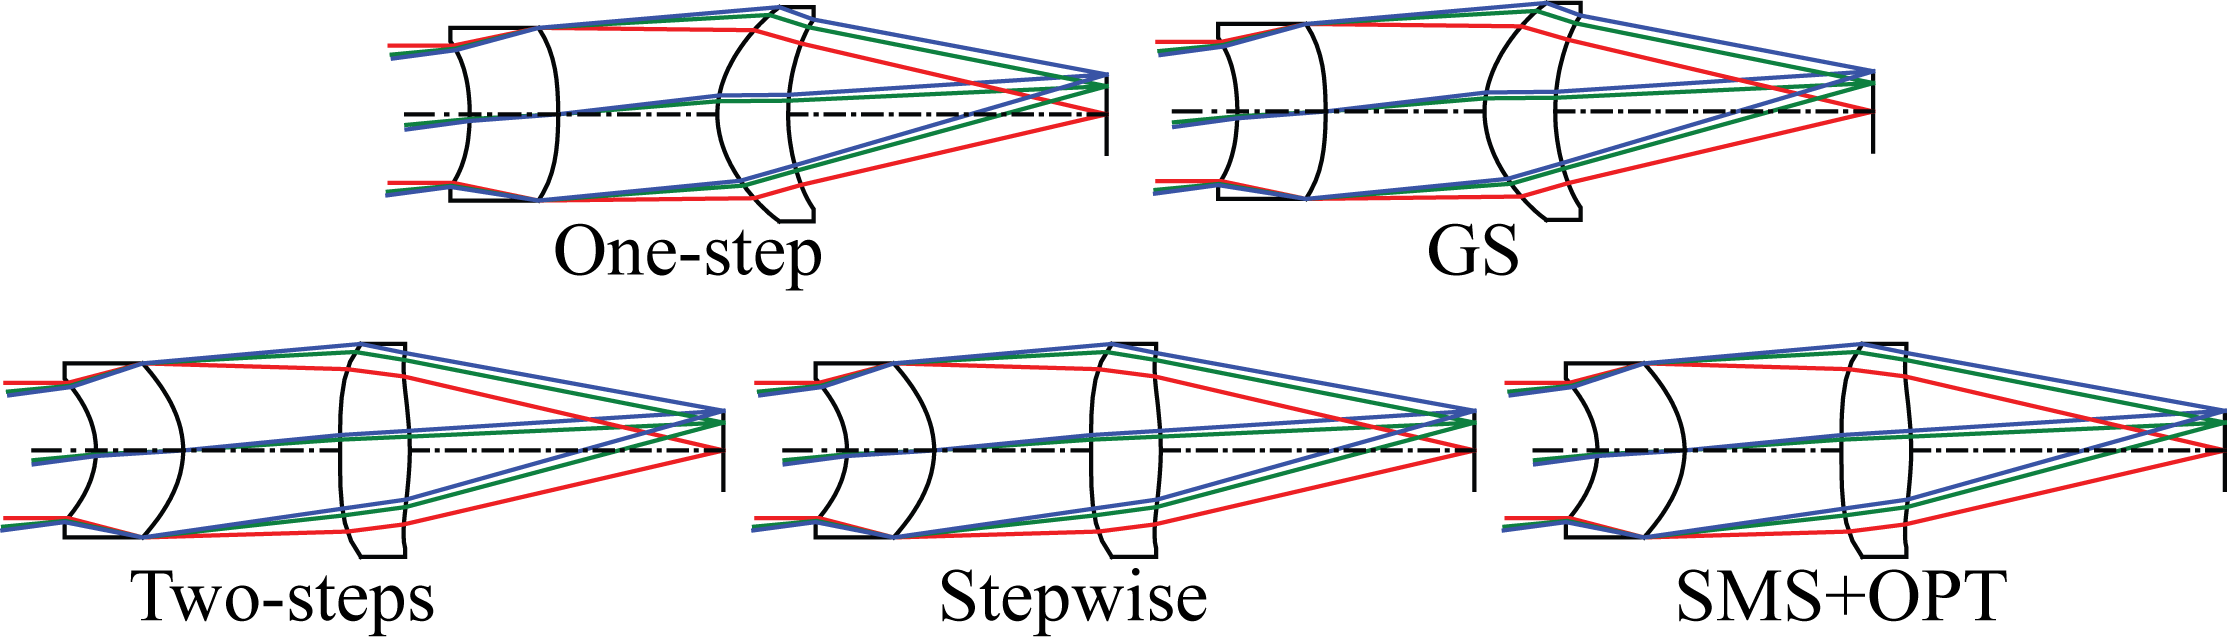
\includegraphics[width=0.8\textwidth]{chapter-5/figures/Figure5_system_plot.png}
    \caption{System 1: the system shapes obtained using different design approaches.}
    \label{fig: fig5_case1_systemplot}
\end{figure}


\begin{figure}[h!]
    \centering
    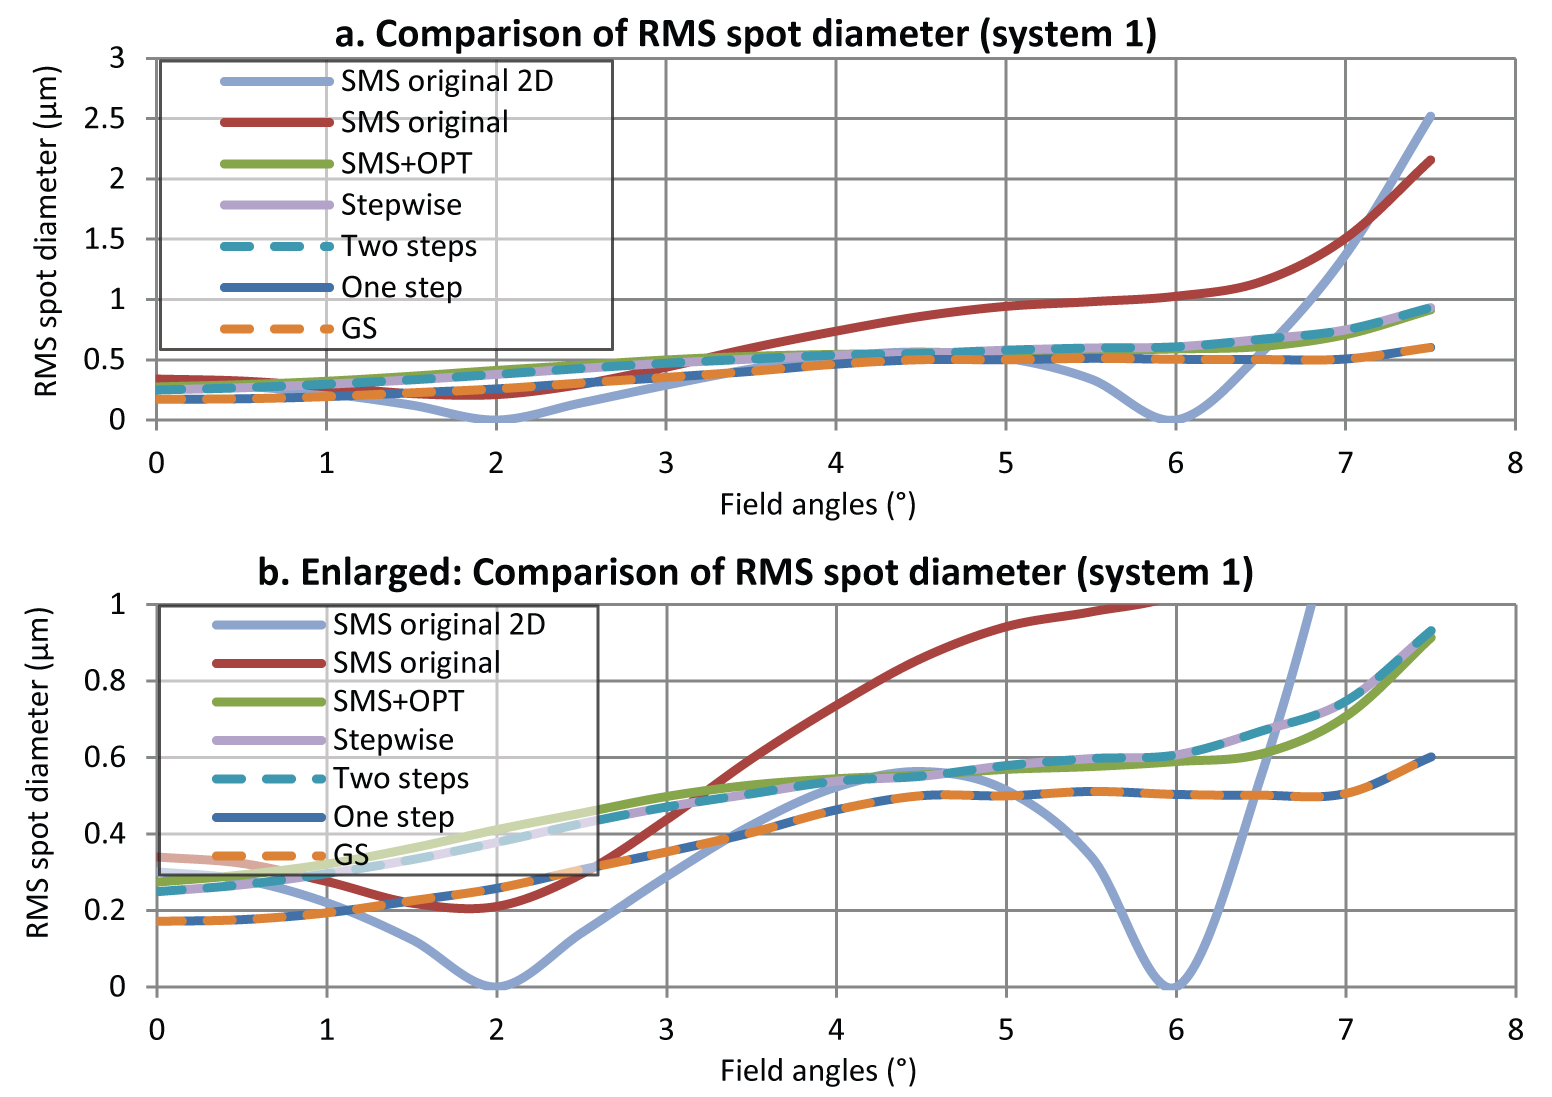
\includegraphics[width=1\textwidth]{chapter-5/figures/Figure6_case1_rmsCurve.png}
    \caption{RMS spot diameter distribution curves for different design approaches considered: complete curves (a); enlarged section (b). The RMS spot diameter values of the starting spherical system vary from 60 to 96 µm and are not presented in the graph.}
    \label{fig: fig6_case1_RMScompare}
\end{figure}

The designed results for system 1 are presented in Figure \ref{fig: fig5_case1_systemplot}. By examining the shapes of the surfaces, we observe two groups of systems: GS and one-step form one group; two-steps, stepwise and SMS+OPT form the other group. This is consistent with the two groups of RMS spot curves in Figure \ref{fig: fig6_case1_RMScompare}. It indicates that solutions from five different strategies end in two different minima in the design space.
In Figure \ref{fig: fig6_case1_RMScompare}, we see that all five systems generated by different approaches show good performance with the maximum RMS spot diameter smaller than 1 μm at the field of 7.5°. The starting SMS system has relatively large RMS spot diameter when the field is increased. Since SMS 2D construction involves only meridional rays,  RMS spot diameter is zero for the design fields ( 2° and 6°) only for those meridional rays (SMS original 2D curve in Figure \ref{fig: fig6_case1_RMScompare}). In Figure \ref{fig: fig6_case1_RMScompare}, a minimum is observed at 2° for the SMS original curve, however, at 6° there is no obvious minimum. Since the RMS spot diameter of SMS original in Figure \ref{fig: fig6_case1_RMScompare} results both from meridional and skew rays, it is reasonable to expect that when the whole pupil is considered, skew rays start to have a larger influence on the spot diameter. The optimization of the SMS constructed system balances the spot diameter over the field with the consideration of the rays from the whole pupil. Except the SMS original and SMS original 2D curve, the curves in Figure \ref{fig: fig6_case1_RMScompare} form two groups, with GS and one-step forming one group, and SMS+OPT, two-steps and stepwise forming the other group, as expected from the system drawings shown in Figure \ref{fig: fig5_case1_systemplot}. The results from GS and one-step are slightly better than the other group.  It can be observed that the curves of GS and one-step almost overlap. The same happens for two-steps and stepwise curves. The overlap of the curves indicates that the optimization strategies lead to the same local minimum in the optimization landscape. The curve of SMS+OPT only has a very small difference shown in field dependence of the RMS compared to the stepwise and two steps curves, which is practically considered as the same local minimum. Because of the smaller values of aperture and field considered here, we have many degrees of freedom, and it is easy to achieve diffraction limited performance. In this situation, several good minima exist in the solution space as illustrated in Figure \ref{fig: fig7_landscape_illus}. Even though the designer still has no control during a one-step optimization, the chance for the optimization reaching a good minimum is higher than in a more difficult design problem.

\begin{figure}[h!]
    \centering
    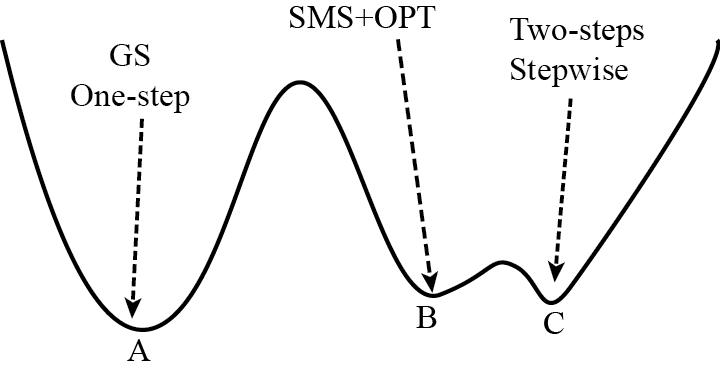
\includegraphics[width=0.6\textwidth]{chapter-5/figures/Fig7_Landscape_illustration_sys1-2.png}
    \caption{An illustration of the design landscape for system 1. We have found three equally good local minima which form two groups. Solution A (MF 0.0301) forms the first group. Solution B (MF 0.0461) and Solution C (MF 0.0450) form the second group.}
    \label{fig: fig7_landscape_illus}
\end{figure}


Figure \ref{fig: fig7_landscape_illus} shows the comparison of the efficiency of the strategies considered in this paper. The GS result is not included because of its very different approach compared to the others: instead of optimizing from one starting point, it searches for different starting points, applies local optimizations to them, and produces multiple solutions \cite{codevmanual} We usually choose the system with the smallest merit function value and perform an extra local optimization to make sure it converges. In this case, we cannot easily use the number of optimization cycles to represent the efficiency of GS. Three solutions were generated with GS after two hours (Intel i5-3470 dual-core @3.20 GHz system). In comparison, it took around 30 seconds for a one-step optimization to run 1000 cycles on the same computer. In Figure \ref{fig: fig8_case1_efficiencyCompare}, the starting points are shown at cycle 0. The two groups have their average MF values as 0.0454 and 0.0301(the MF value of the GS result is 0.0301). An MTF analysis shows that all five systems are diffraction limited at the wavelength used here. This is consistent with our statement that the design problem is easy and multiple equally good minima are present. Therefore, this example shows that in simple design problems like system 1 simple methods can easily lead to a good solution. 

System 1 has a relatively small pupil and field, which reduces the difficulty of the design. With the same approach, we used SMS to construct system 2, which has both a larger pupil and field of view. Figure \ref{fig: fig9_case2_systems} shows the five plots of the systems produced by five different optimization approaches. In contrast with the solutions of system 1 in Figure \ref{fig: fig5_case1_systemplot}, four different system shapes are obtained, where stepwise and SMS+OPT resulted in the same system shape. The operation with GS for system 2 was not as straightforward as that for system 1. It is worth noting that the aperture stop of system 2 is placed in between the two lens element as shown in Figure \ref{fig: fig9_case2_systems}. This is to impose the that when using SMS only four ray bundles are used for a four-surface design. Other positions of the aperture stop lead to the use of more than four ray bundles as shown in \cite{BenitezSPIE2014}\cite{FDuerrOE2013}\cite{FDuerrOE12} and it will not be consistent with the SMS design approach in system 1.

\begin{figure}[h!]
    \centering
    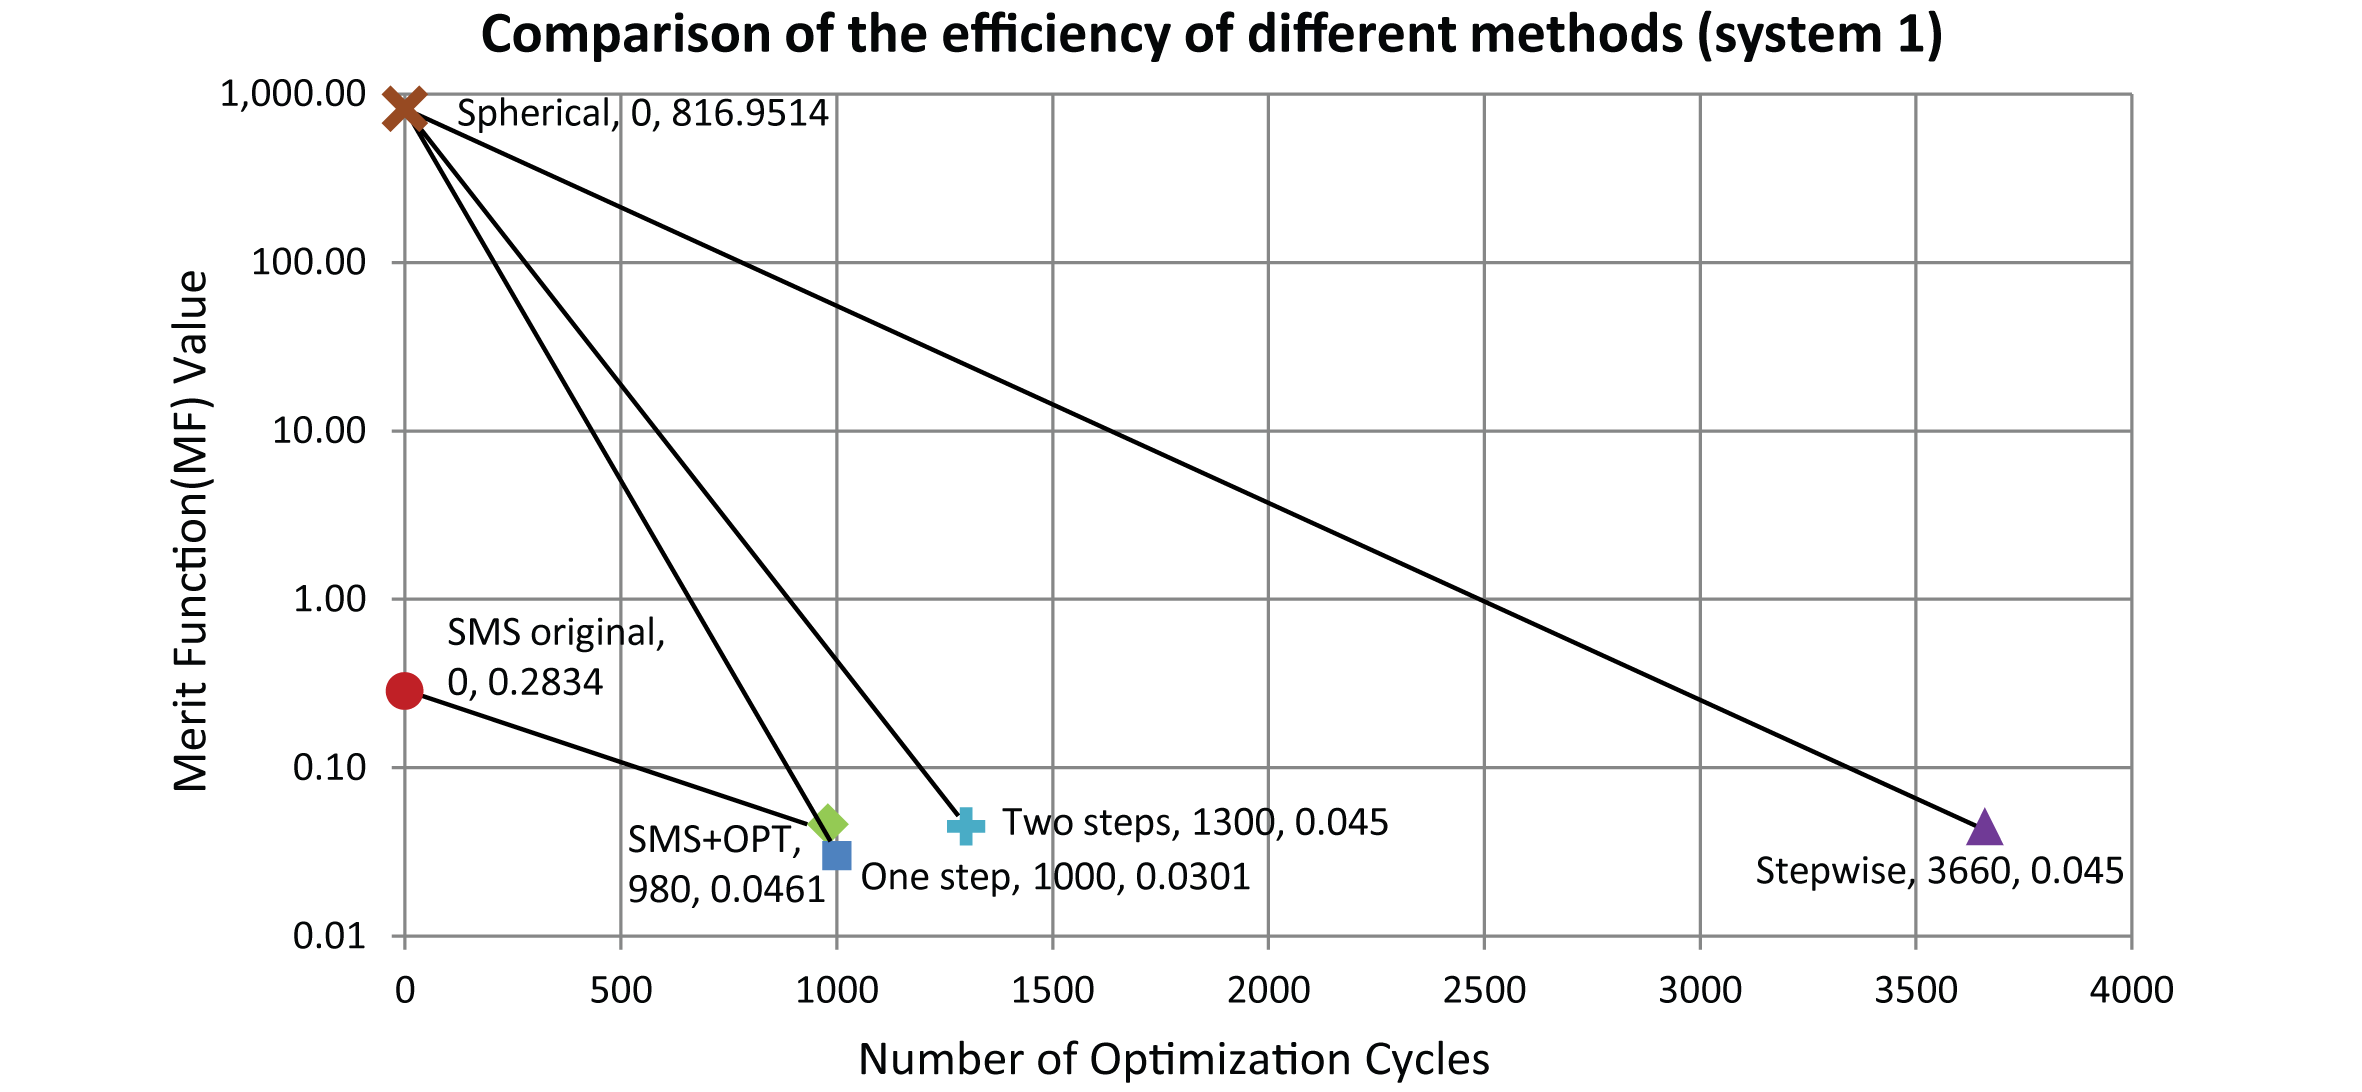
\includegraphics[width=1\textwidth]{chapter-5/figures/Figure8_OE340147.png}
    \caption{Comparison of the efficiency of different design methods analyzed, evaluated as the merit function value versus the number of cycles performed. The merit function value of the resulting system from GS is 0.0301.}
    \label{fig: fig8_case1_efficiencyCompare}
\end{figure}

Optimization with conic constants as variables ended with systems having an extremely large conic constant. Therefore, we first fixed the conic constant on all the surfaces to -1, and ran the GS which resulted in twelve solutions. After that, the conic constants on all the surfaces of the twelve systems were freed at once as variables. Subsequent local optimization, which is the same as the one used in the other four strategies, was applied to each of the twelve systems. The system with the smallest MF value was chosen as the final result. In Figure \ref{fig: fig10_case2_rmsCurvecompare}, the curves of RMS spot diameter can be again divided into two groups. One-step and two-steps optimization generate poorer solutions than the rest of the approaches. SMS with optimization, stepwise optimization and GS obtain good solutions with close RMS dependence along the field (Figure \ref{fig: fig10_case2_rmsCurvecompare}(b)). Consistent with the same system shape in Figure \ref{fig: fig9_case2_systems}, the RMS curves of SMS+OPT and stepwise in Figure \ref{fig: fig10_case2_rmsCurvecompare} almost overlap each other. On the other hand, the result of GS with a different system shape produces a different RMS curve, where the RMS spot diameter is bigger under 7.8° and smaller above 7.8°.

\begin{figure}[h!]
    \centering
    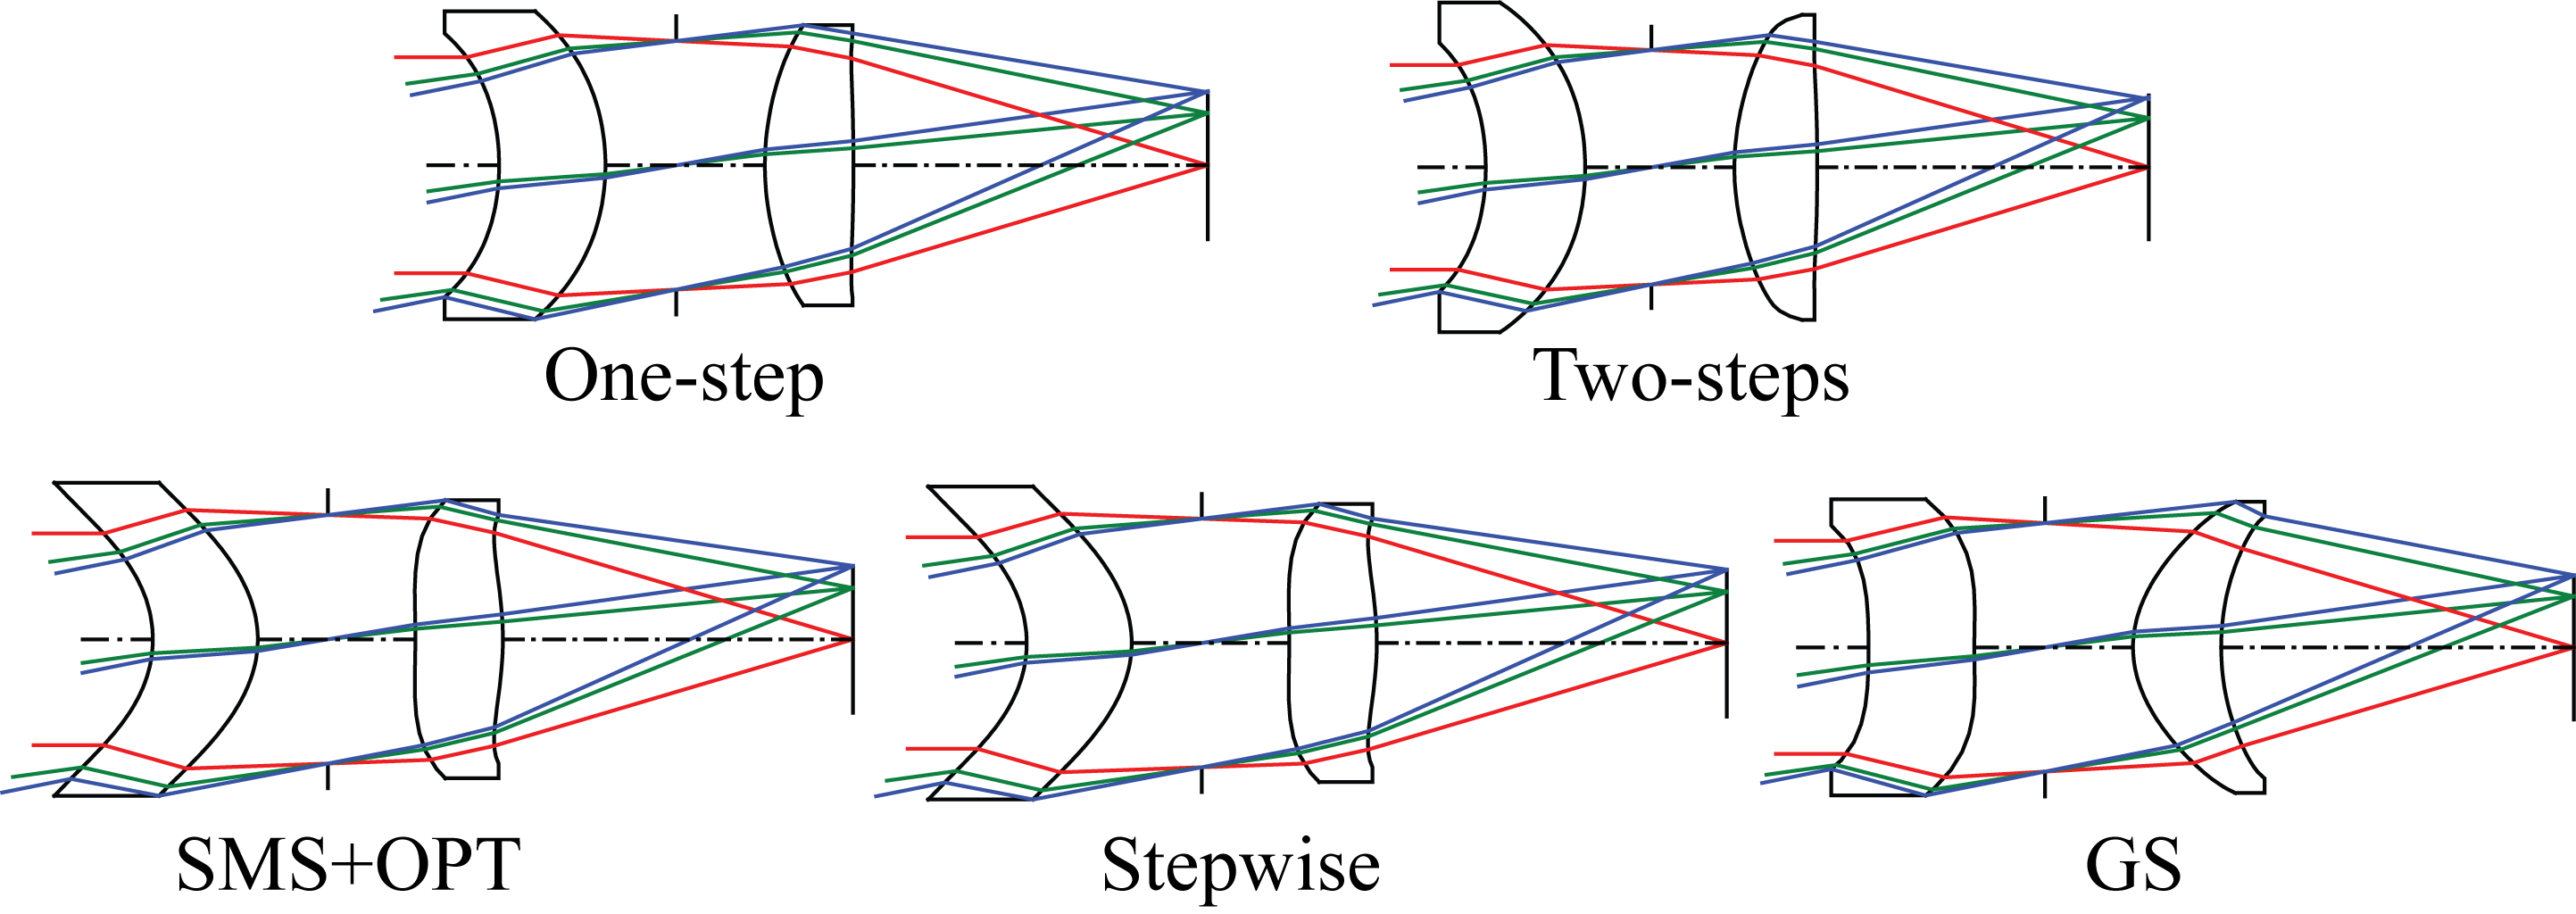
\includegraphics[width=0.8\textwidth]{chapter-5/figures/Figure9_system2_solutions.png}
    \caption{System 2: the system shapes obtained using different design approaches.}
    \label{fig: fig9_case2_systems}
\end{figure}

Figure \ref{fig: fig11_case2_efficiencyCompare} shows the comparison of the efficiency of different methods. Stepwise needs a large number of optimization cycles (8100 cycles) to converge. With a similar merit function value, fewer optimization cycles are needed for SMS optimization. This shows the SMS constructed starting point is closer to the minimum in the optimization landscape. Both one-step and two-steps optimization are trapped in poor solutions with MF values at least nine times of the best solution. 
From the two examples we studied, to design a simple system with small field and aperture, all approaches including a one-step optimization were able to obtain good solutions. However, when the field and aperture increased, simple strategies like one-step and two-step started to fail by getting trapped in poor local minima as shown in the example of system 2. A stepwise approach leads to a good local minimum with a large number of optimization cycles. An SMS constructed starting point located closer to a good solution shows its advantage in both cases where fewer optimization cycles are needed to reach a good local minimum.

\begin{figure}[h!]
    \centering
    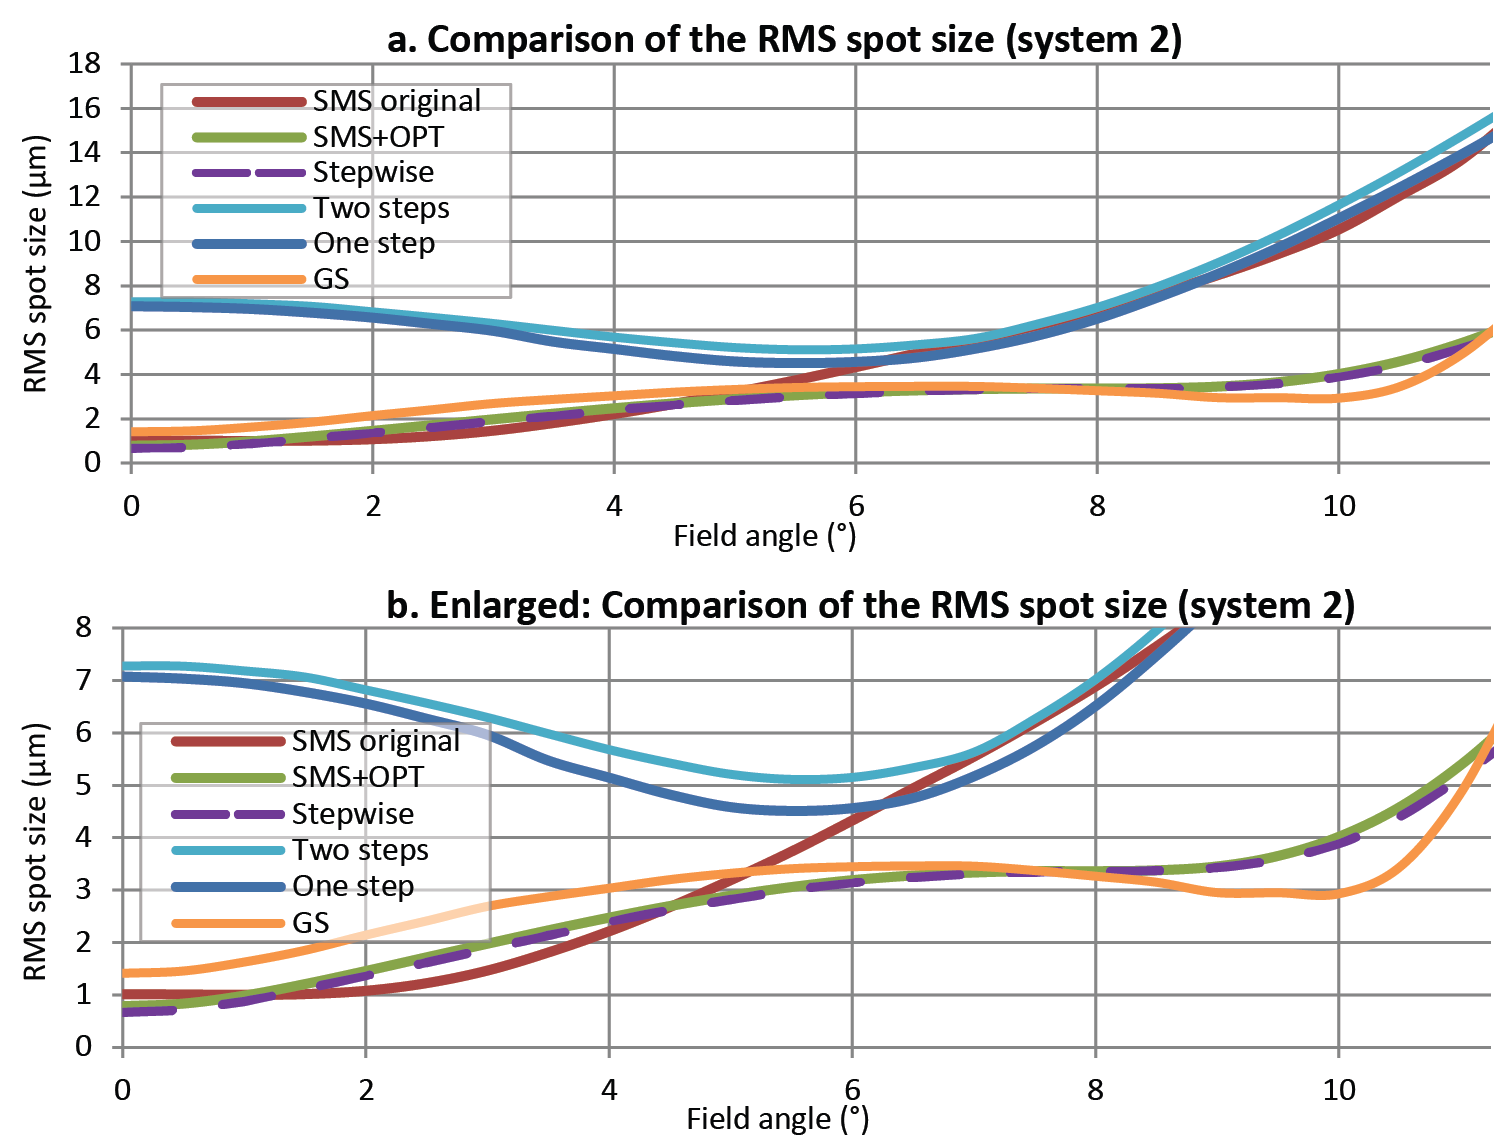
\includegraphics[width=1\textwidth]{chapter-5/figures/Fig10_case2_rms.png}
    \caption{RMS spot diameter curves for second system using different design approaches: complete curves (a); enlarged section (b). The RMS spot diameter values of the starting spherical system vary from 124 to 142 µm from the center to the full field and are not shown in the graph.}
    \label{fig: fig10_case2_rmsCurvecompare}
\end{figure}

\begin{figure}[h!]
    \centering
    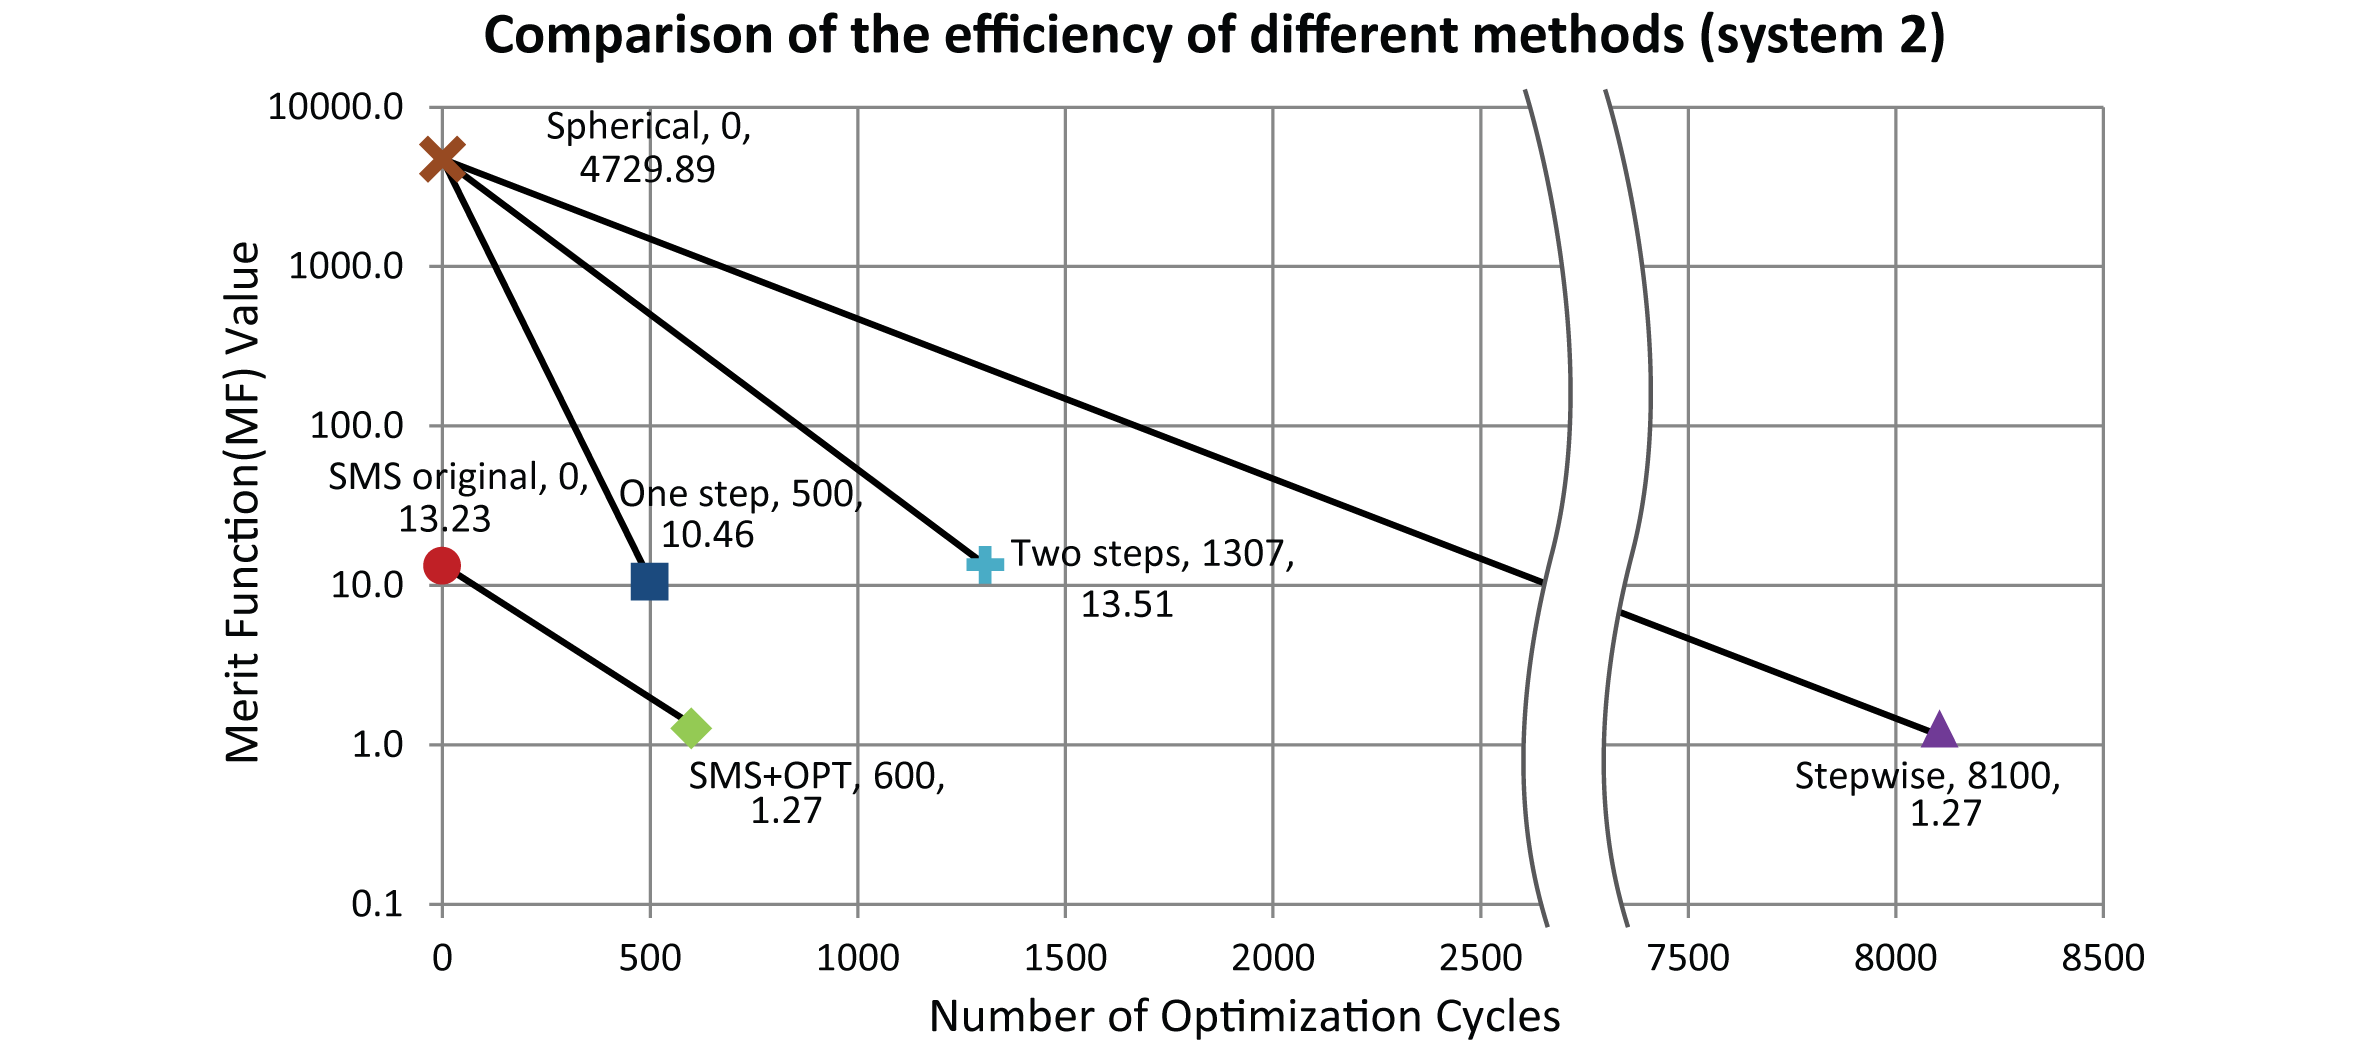
\includegraphics[width=1\textwidth]{chapter-5/figures/Figure11_OE340147.png}
    \caption{Comparison of the efficiency of different design methods. The starting points are shown at zero cycles and are connected with the straight lines with the results obtained using different design methods. The merit function value of the GS result is 1.03.}
    \label{fig: fig11_case2_efficiencyCompare}
\end{figure}

\section{Design landscape for aspheric systems}
In our examples, we have noticed that when the aspheric variables are not introduced, there is only one solution in the optimization landscape given the boundary condition, where rays can be traced. However, when aspheric coefficients are added, new minima start to appear. 

\begin{figure}[h!]
    \centering
    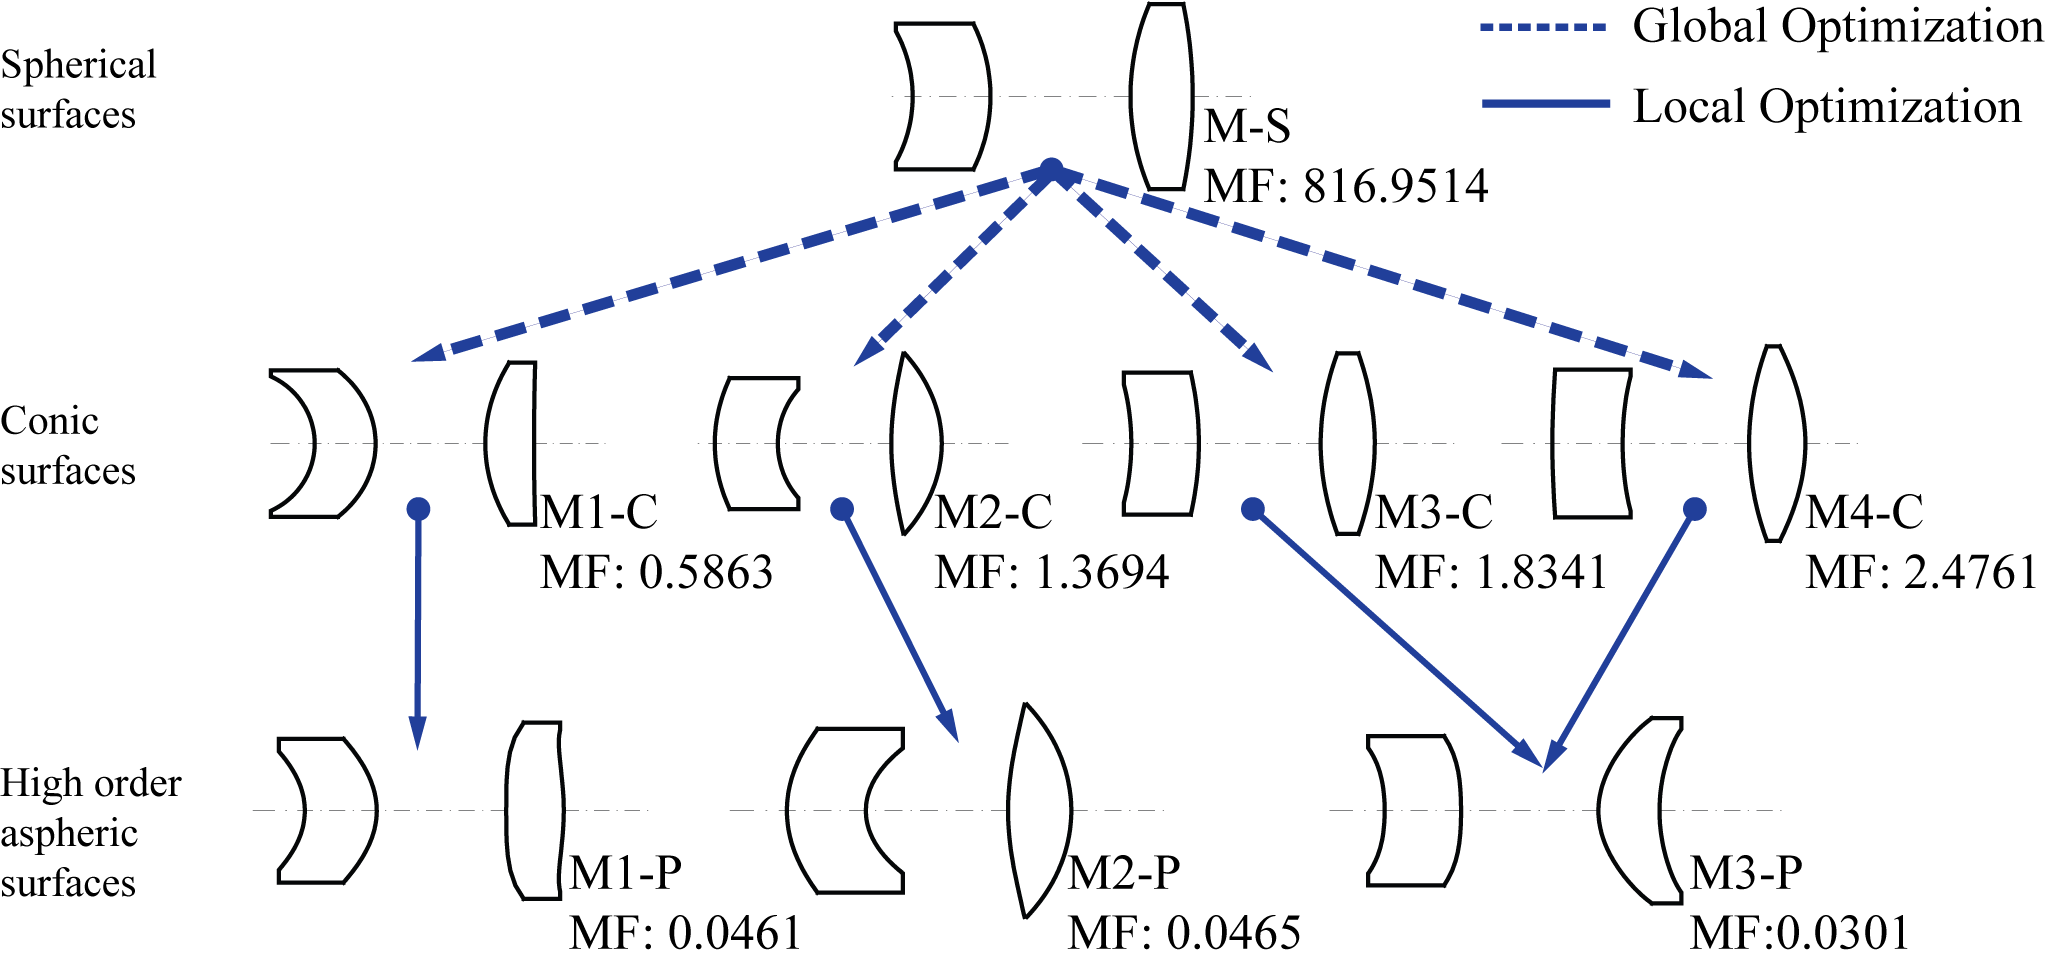
\includegraphics[width=0.8\textwidth]{chapter-5/figures/Fig12_System1_structure.png}
    \caption{Evolution of the minima with the change of aspheric coefficients (system 1). Four minima are found with conic surfaces. They become three minima when optimized with aspheric coefficient up to 12th order. All three are found with the different approaches we used. M1-P and M3-P are the two solutions previously found with the different approaches(Figure \ref{fig: fig5_case1_systemplot}). }
    \label{fig: fig12_case1_optStruc}
\end{figure}

After adding the conic constant as a variable, multiple minima appear in the design landscape. We used GS of CODE V, in this case, to search for different solutions. For system 1, we have found four minima (Figure \ref{fig: fig12_case1_optStruc}), and for system 2 three (Figure \ref{fig: fig13_case2_optStruc}). 
The following step included adding all other higher-order aspheric coefficients at once to locally optimize the systems from the conic minima. For system 1, four different minima in conic space converge to three minima. In Figure \ref{fig: fig12_case1_optStruc}, two of the three minima (M1-P, M3-P) are identical to the ones shown in Figure \ref{fig: fig5_case1_systemplot}, and M2-P was also found by the GS, which is not shown in Figure \ref{fig: fig5_case1_systemplot}. For system 2, three solutions result from the three conic minima. In Figure \ref{fig: fig13_case2_optStruc}, M1-P and M2-P are same as the results of the two-steps approach and the SMS with optimization respectively. M3-P is a poor local minimum which is not found by the approaches we used.

\begin{figure}[h!]
    \centering
    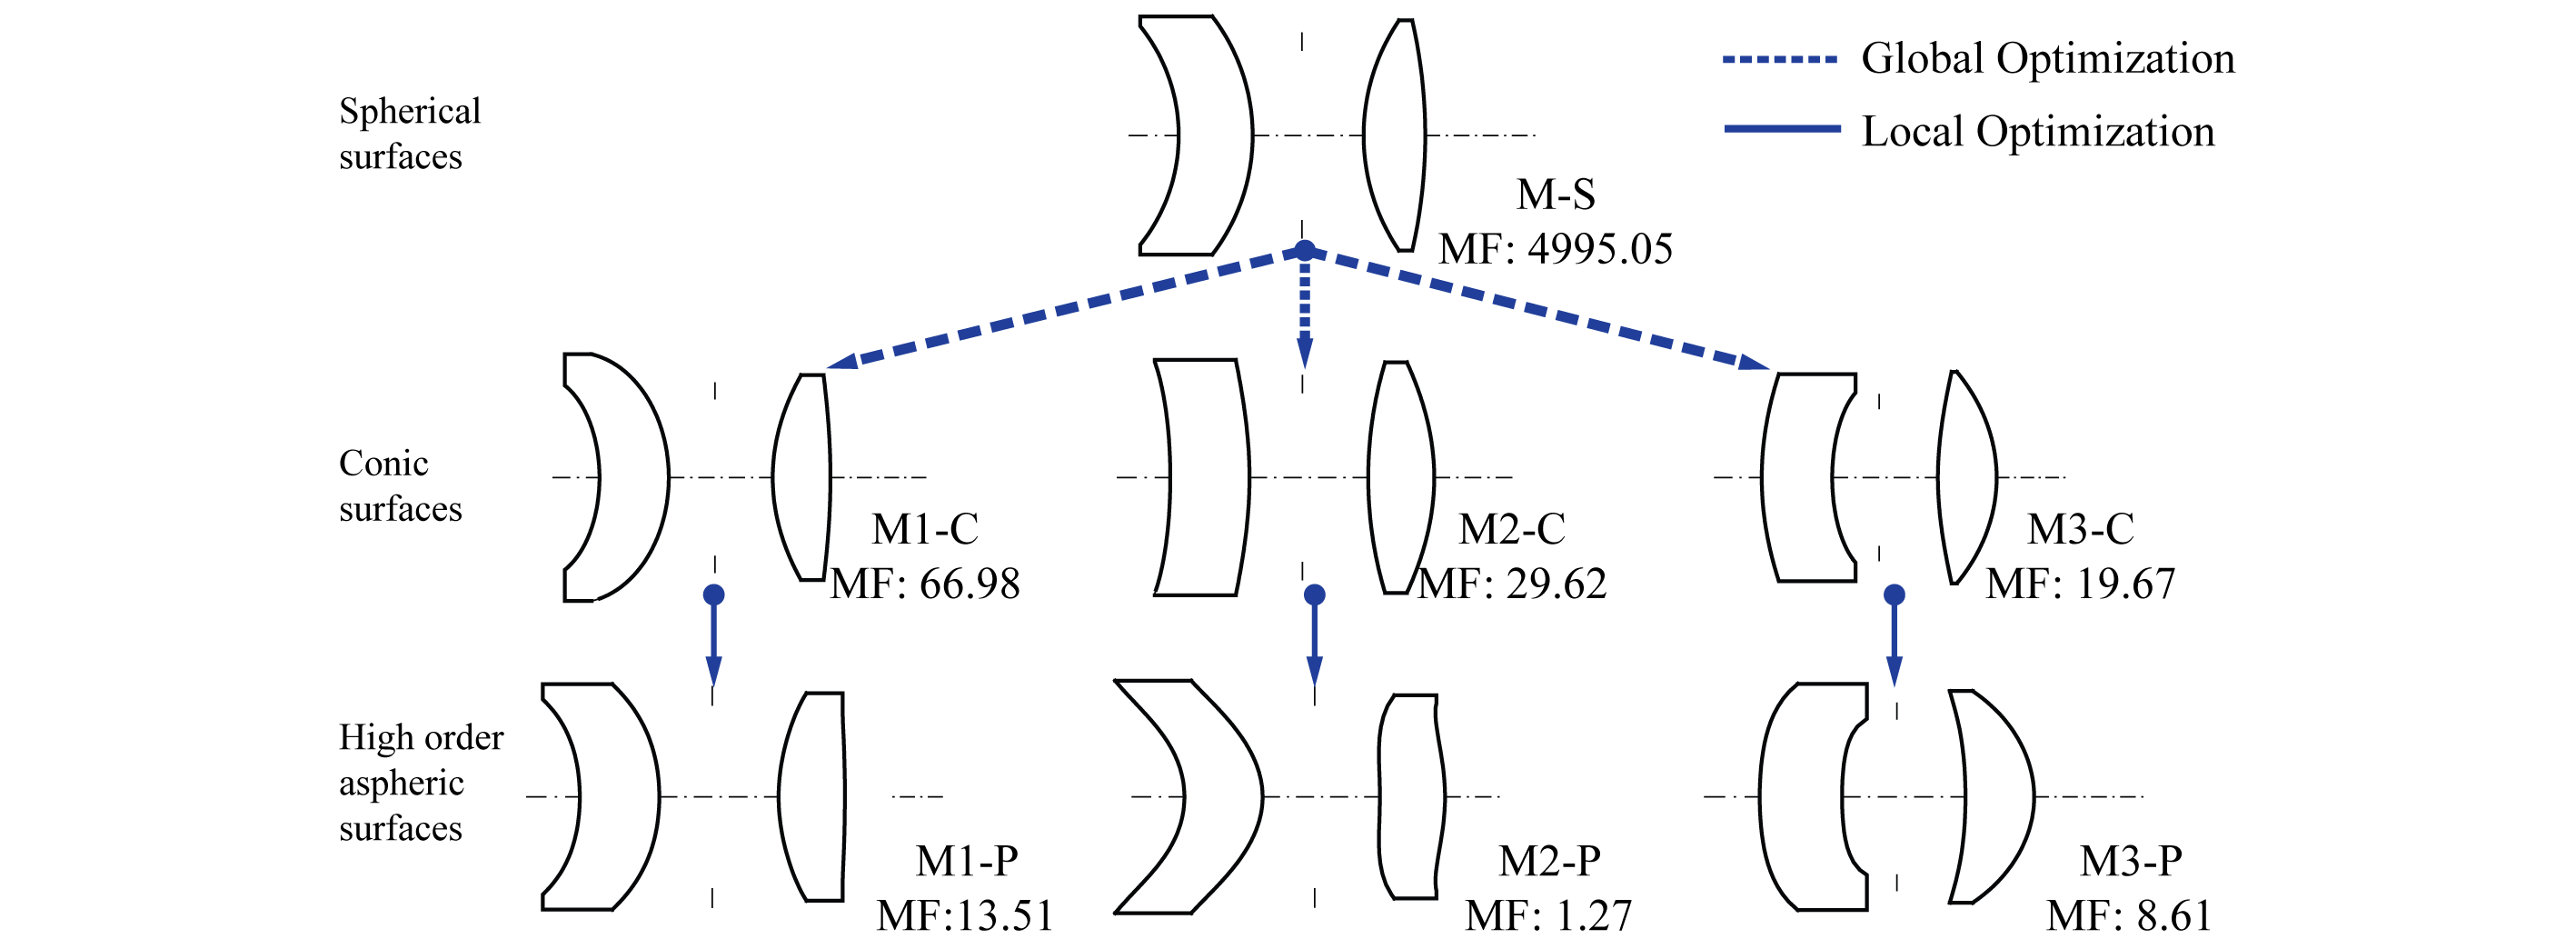
\includegraphics[width=1\textwidth]{chapter-5/figures/Fig13_OE340147.png}
    \caption{Figure \ref{fig: fig13_case2_optStruc}. Evolution of the minima with the change of aspheric coefficients (system 2). Three minima are found with conic surfaces. Adding higher-order aspheric coefficients (up to 16th order) to these minima results in three different solutions. M1-P is the solutions found by the two-steps approach, and M2-P is the solution found by the SMS with optimization in Figure \ref{fig: fig9_case2_systems}}
    \label{fig: fig13_case2_optStruc}
\end{figure}

The results show the dynamic behavior of the optimization landscape. Namely, the number of minima may change depending on the number and type of variables used. In the two systems we have studied in this paper, the introduction of the conic surface creates new minima in the design landscape, and adding higher-order aspheric coefficient deepens the original minima. For a simple system, adding higher-order aspheric coefficients does not complicate the landscape. With local optimization, the conic solutions lead to the good solutions with higher-order aspheric coefficients. In the case of system 2, where aperture and field are large, adding higher-order aspheric coefficients complicates the landscape by creating new local minima. That is the reason why simple strategies are trapped in poor local minima. In both cases, the SMS constructed starting points are already close to one of the good local minima in the landscape. Therefore, local optimizations with few optimization cycles lead to good solutions.

\section{Conclusions}
Two different optical systems comprising of two lenses were analyzed. In the analysis of the design landscape of the systems, we have observed that with aspherising the surfaces, new minima emerge into the landscape. In both examples, introducing lower order aspheric coefficients (conic constant) to all the surfaces brings new local minima into the landscape, and adding higher-order aspheric coefficients deepens the minima. In a simple design with both small aperture and field (system 1), adding higher-order coefficients does not complicate the landscape by creating new local minima. In contrast, for a different design with large aperture and field (system 2), higher-order aspheric coefficients introduce new local minima, where a design process can be trapped.
We have compared SMS design approach with other design techniques to design and optimize the two systems. In the case of the simpler system (system 1) considered, all design techniques including a one-step optimization found solutions close to diffraction limit. Nevertheless, surface shapes of the final designs were different which suggested that their optimization paths ended in different basins of attractions. 
In the second design example (system 2) analyzed, SMS with posterior optimization, the stepwise approach and GS found optimal solutions. Carefully analyzing the three results obtained, we conjectured that they belong to two different minima. Since designing system 2 is more demanding than system 1, less robust methods such as one-step optimization and two-steps optimization did not lead to good minima. Despite that three approaches found good solutions, stepwise optimization usually takes the largest amount of optimization cycles. GS works well with the simple case. However, for system 2, effective constraints (in this case, fixed conic constant) and further optimizations are needed to be implemented into GS to get reasonable solutions. In practice, lens design problems are very different depending on the application and constraints. While we cannot guarantee that SMS will find good solutions in other design problems, the present results are encouraging. In both cases, SMS with posterior optimization can find good solutions, and we can see from Figure \ref{fig: fig8_case1_efficiencyCompare} and Figure \ref{fig: fig11_case2_efficiencyCompare} that in the two examples considered, SMS constructs good starting points which are close to the good solutions. It is our hope that with such comparative studies, we can provide the designers with insight into the characteristics of different methods.


\references{dissertation}

